%
% General structure for the revdetua class:
%
\documentclass[...]{revdetua}
\usepackage{graphicx}
\usepackage{float}

%
% Valid options are:
%
%   longpaper --------- \part and \tableofcontents defined
%   shortpaper -------- \part and \tableofcontents not defined (default)
%
%   english ----------- main language is English (default)
%   portugues --------- main language is Portuguese
%
%   draft ------------- draft version
%   final ------------- final version (default)
%
%   times ------------- use times (postscript) fonts for text
%
%   mirror ------------ prints a mirror image of the paper (with dvips)
%
%   visiblelabels ----- \SL, \SN, \SP, \EL, \EN, etc. defined
%   invisiblelabels --- \SL, \SN, \SP, \EL, \EN, etc. not defined (default)
%
% Note: the final version should use the times fonts
% Note: the really final version should also use the mirror option
%

\begin{document}

\Header{1}{25}{novembro}{2022}{0}
% Note: the month must be in Portuguese

\title{Finding the Minimum Weighted Closure of a Graph using Exhaustive Search and a Greedy Algorithm}
\author{Eduardo Santos, nºmec 93107, eduardosantoshf@ua.pt} % or \author{... \and ...}
\maketitle

\begin{abstract}
The objective of this assignment was to find a minimum weighted closure for a given vertex-weighted directed graph \textit{G(V, E)}, with \textit{n} vertices and \textit{m} edges. Exhaustive Search and Greedy Algorithms were used to solve this problem, with the solution explained in this paper, and both approaches being compared in terms of execution time, as well as complexity. The computations were made using a variety of parameters, which will also be referred on the following sections.
\end{abstract}

\section{Introduction}

A closure of \textit{G} is a set of vertices \textit{C}, such that no edges leave \textit{C}. The weight of a closure is the sum of its vertices’ weights. A \textbf{minimum weight closure} is a closure whose total weight is as small as possible. Both algorithms used computed the minimum weighted closure of a given graph, with each approach and its parameters explained later on.

\section{ Problem Description}

To solve this problem, the first thing to do was to create a random graph, so that it could be used to compute the minimum weighted closure. To do this, the NetworkX\cite{networkx} library was used, which is a useful tool for creating, manipulating, and studying the structure, dynamics, and functions of complex networks, or graphs.
To better understand this problem, let's consider a graph with 5 nodes and 5 edges, represented in the figure below. In this particular case, and in order to facilitate the explanation, a graph with multiple closures was used. Let's also consider each node's number as its weight. 

\begin{figure}[!htb]
    \centering
    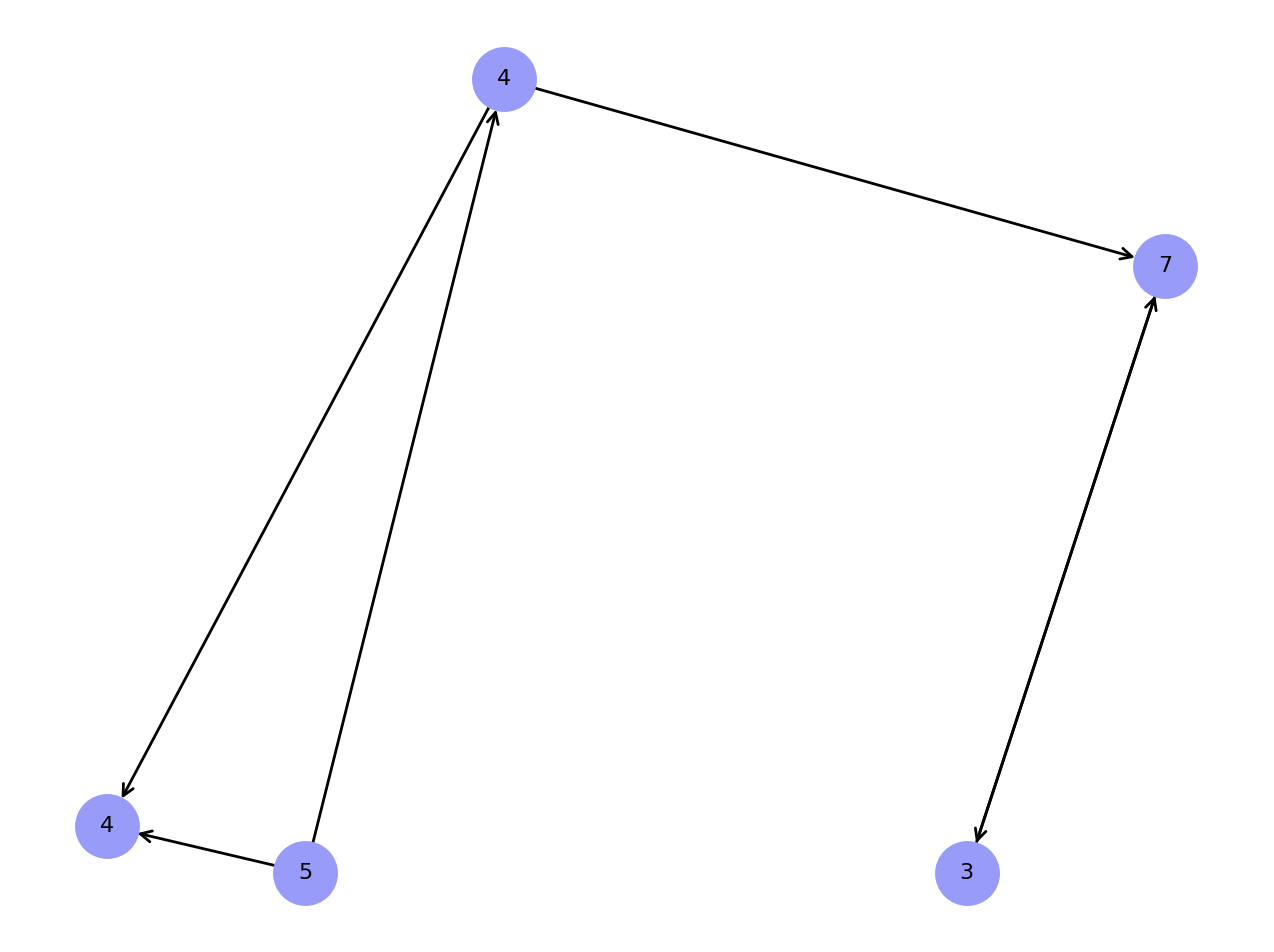
\includegraphics[width=0.75\columnwidth]{./figures/simple_graph.png}
    \caption{Example of a Simple Graph}
    \label{fig: Simple Graph}
\end{figure}

\newpage

The graph above has 5 sets that are closures:

\begin{itemize}
    \item 4 (weight: 4)
    \item 3, 7 (weight: 10)
    \item 3, 7, 4 (weight: 14)
    \item 3, 7, 4, 4 (weight: 18)
    \item 3, 7, 4, 4, 5 (whole graph) (weight: 23)
\end{itemize}

Therefore, the minimum weighted closure of this graph is 4, as it represents the minimum sum of closure vertices' weights.

\section{ Implementation Description}

Running the main program, there are a few flags that can be used, depending on what we wish to compute, etc.

\begin{figure}[!htb]
    \centering
    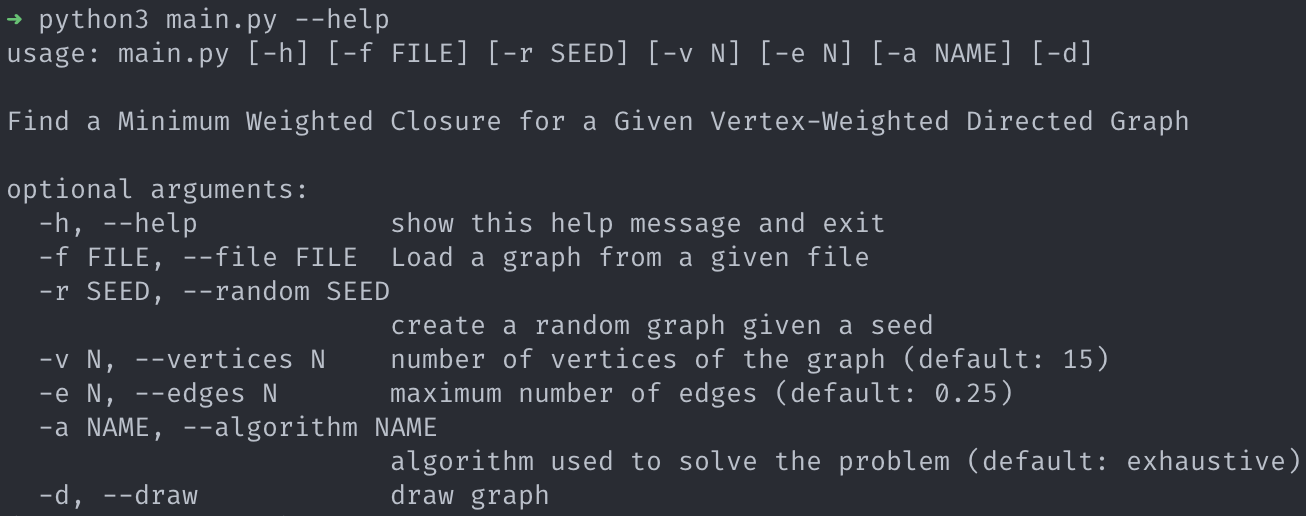
\includegraphics[width=1\columnwidth]{./figures/program_help}
    \caption{Help Menu of the Main Program}
    \label{fig: Help Menu}
\end{figure}

To compute using both the exhaustive and the greedy search, there are two options to create a graph. Using the \textbf{-f} flag, a graph can be read from a file, with the following format:
\begin{verbatim}
4
1 1 9
1 2 5 3
2 3 4 1 2
3 5 7 2
\end{verbatim}

The first line represents the number of nodes in the graph, and each following line represents the \textbf{\textit{x} coordinate}, \textbf{\textit{y} coordinate}, \textbf{node weight}, and the \textbf{node(s) to which it connects}, all separated by spaces.

Using the \textbf{-r} flag, the program generates a random graph, using a student number as a seed, and the number of nodes given by the \textbf{-n} flag. Each node's coordinates are randomly generated values from 1 to 20, and it only adds a node if the point did not already exist. Also, when generating random edges, the flag \textbf{-e} is used to set the maximum number of edges of the graph to be generated. For the computations, which will be discussed later in this paper, the values 12.5\%, 25\%, 50\%, and 75\% will be used as the maximum number of edges.

The \textbf{graph.py} contains the \textbf{Graph}, \textbf{GraphDrawer}, \textbf{ExhaustiveSearch}, and the \textbf{GreedySearch} classes. In the \textbf{Graph} class, there are two methods to help with the definition of a graph:

\begin{itemize}
    \item \textit{add\_node(self, node: Point, weight: int)} - this method saves the nodes in a dictionary, with the node coordinates as key, and the node's weight as value.
    \item \textit{add\_edge(self, node1: Point, node2: Point)} - this method saves the edges also on a dictionary, with \textit{node1} as key, and adding the \textit{node2} to the first one's key list. This is helpful when the problem uses a directed graph, because of the starting/ending node of an edge matter, regarding its order.
\end{itemize}

There is also the flag \textbf{-a} to choose between the exhaustive and the greedy algorithms, with the first one being the default one, and the \textbf{-d} flag, which allows drawing the graph, using the Matplotlib\cite{matplotib} library.

In the graph below, the minimum weighted closure is presented with the color green. This solution was computed using the exhaustive algorithm.

\begin{figure}[!htb]
    \centering
    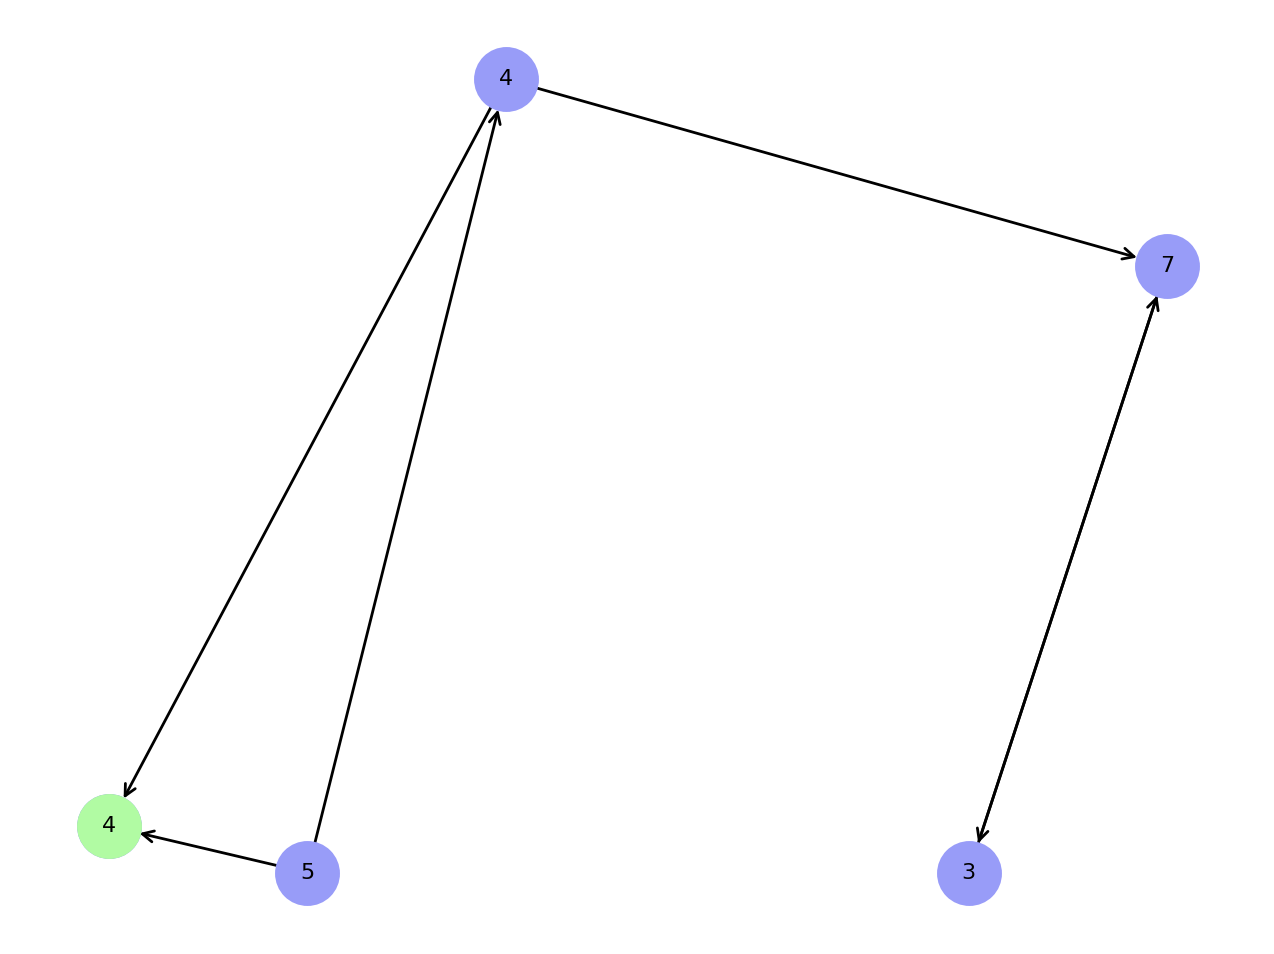
\includegraphics[width=0.75\columnwidth]{./figures/simple_graph_exhaustive_solution.png}
    \caption{Minimum Weighted Closure Using the Exhaustive Algorithm}
    \label{fig: Minimum Weighted Closure Using the Exhaustive Algorithm}
\end{figure}

On the contrary, using the greedy algorithm, a different solution was found. This solution's minimum weighted closure is also represented with the color green, in the graph below.

\begin{figure}[!htb]
    \centering
    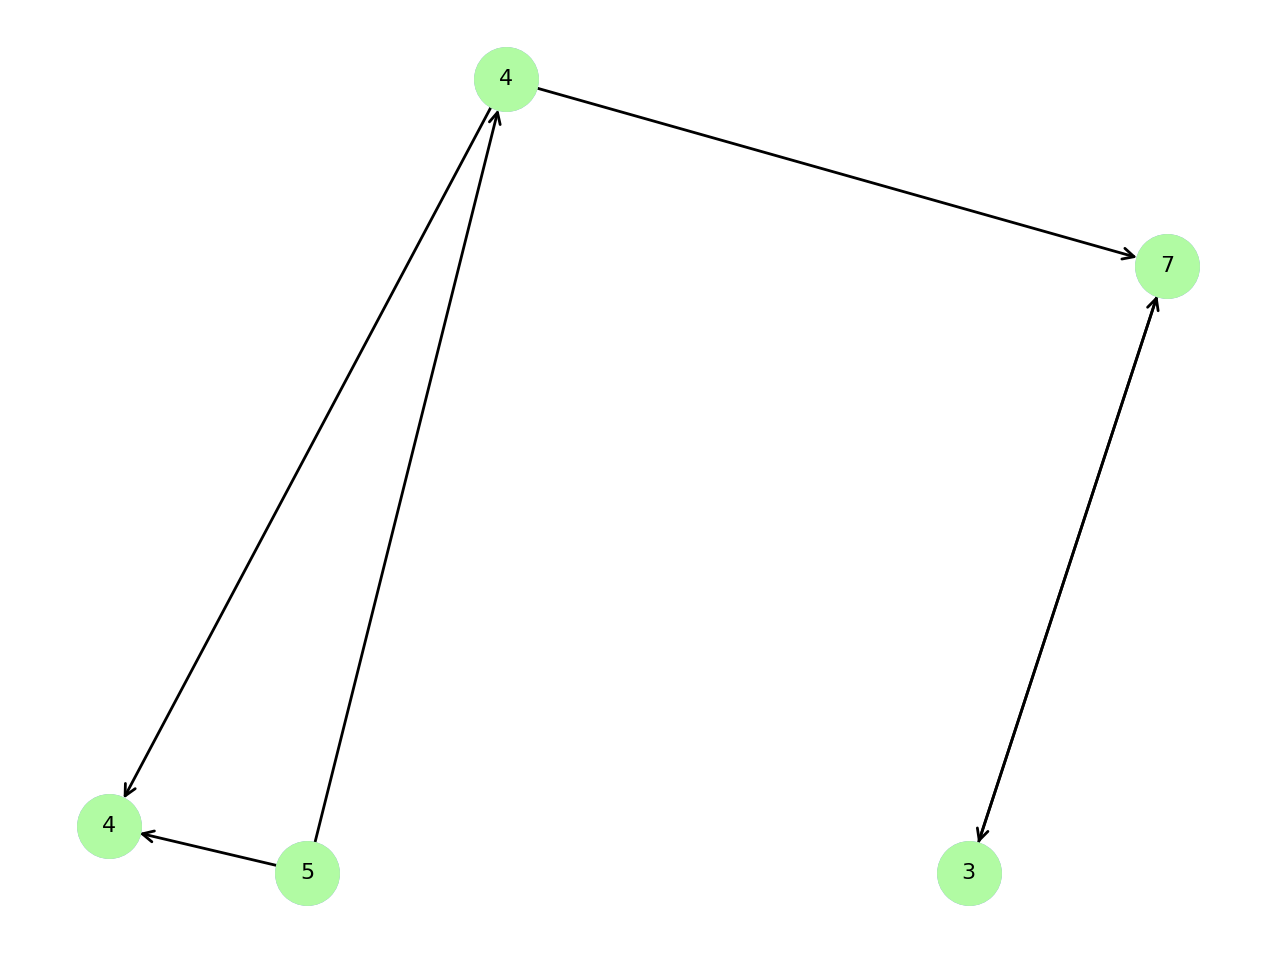
\includegraphics[width=0.75\columnwidth]{./figures/simple_graph_greedy_solution.png}
    \caption{Minimum Weighted Closure Using the Greedy Algorithm}
    \label{fig: Minimum Weighted Closure Using the Greedy Algorithm}
\end{figure}

\newpage

In this specific case, the whole graph is considered by the algorithm as the minimum weighted closure. The reason for that will be later on explained.

\subsection{Exhaustive Search}

Regarding the exhaustive search, firstly the power set of the set of nodes is computed. The power set of a set S is the set of all subsets of S, including the empty set and S itself, of size 1 to N, where N is the total number of nodes. In this case, every subset is considered a possible closure. Then, for every subset, \textit{C}, it is necessary to check if there are any edges for other nodes that are not in \textit{C}. If this happens, then \textit{C} is not a closure, if not, then the subset is added to the \textit{closures} list. After having all closures, every subset node's weight is added, and the closure with the smallest sum is considered the minimum weighted closure.

\subsubsection{Formal Computational Complexity Analysis}

% O(n2^n) para o exhaustive e O(n^2) para o greedy

Performing a formal computational analysis of the exhaustive search algorithm, regarding the time complexity, the complexity would be \textit{O(2$^N$ * N)}, since it is the sum of all combinations of nodes, which can be seen as the sum of numbers of \textit{nth} row of Pascal's triangle. As we also need to iterate over all the nodes of a possible closure, this step increases the complexity by multiplying it by \textit{N}, obtaining the final complexity, mentioned above.

\subsection{Greedy Search}

Regarding the greedy search, instead of computing all subsets for the set of the graph's nodes (power set), the solution is obtained by starting on the node which has the smallest weight. Firstly, the nodes are ordered in descending order by their weight. Then, the node with the lowest weight is put in a set as a possible closure, and then the algorithm verifies if the set is, in fact, a closure. If not, the next node with the smallest weight is added to the possible closure set, and the process is repeated. Sometimes, if all the nodes are added to the set, then the whole graph is considered a closure, and so, the solution to the problem.

\subsubsection{Formal Computational Complexity Analysis}

%eu meti (N(N + 1))/2  já a tentar calcular o numero de vezes que faziam os 2 fors em conjunto

%como dá append dentro do 1º for

%o 2o for na primeira vez ia percorrer um ciclo, depois davas append e por isso percorria agora 2 ciclos, dps 3, e assiam adiante

%dps só vi a formula da soma de uma sequencia de numeros naturaris, q é (N(N + 1))/2, e em big oh notation dava O(n^2)

Performing a formal computational analysis of the greedy search algorithm, regarding the time complexity, the complexity would be \textit{O(N$^2$)}, since the complexity of the nodes dictionary sort is \textit{O(N * $\log N$)}, and the complexity of the algorithm itself is given by \textit{(N * (N + 1)) / 2}, which can be expressed as:

\[
    \frac{N * (N + 1)}{2} = \frac{N^2 + N}{2}
\]

The expression above in Big O notation represents \textit{O(N$^2$)}. Adding both complexities we obtain the complexity of the algorithm:

\[
    O(N * \log N) + O(N^2) = O(N^2)
\]

\newpage

\section{Results and Discussion}

To better understand the performance of both algorithms, as well as to compare each other, several plots were drawn. Both the exhaustive and the greedy algorithms were compared using three parameters: number of iterations, number of solutions found, and execution time. 
For each algorithm, the results were computed using successively larger random graphs with 1 to 20 nodes. With 20 nodes, the algorithm took approximately twenty minutes to compute the results, therefore, 20 was the maximum number of nodes used for the computations. Another important thing to notice is that, as the graphs were randomly generated, the directions of the nodes are also random, which means that there is a slightly higher probability that some graphs' minimum weighted closure is the entire graph. As previously mentioned, to compute the solutions, the maximum number of edges was 12.5\%, 25\%, 50\%, and 75\%. The results presented in the following plots were calculated using 25\% as the maximum number of edges. All of the results can be found in the \textbf{results/} folder.

\begin{figure}[H]
    \centering
    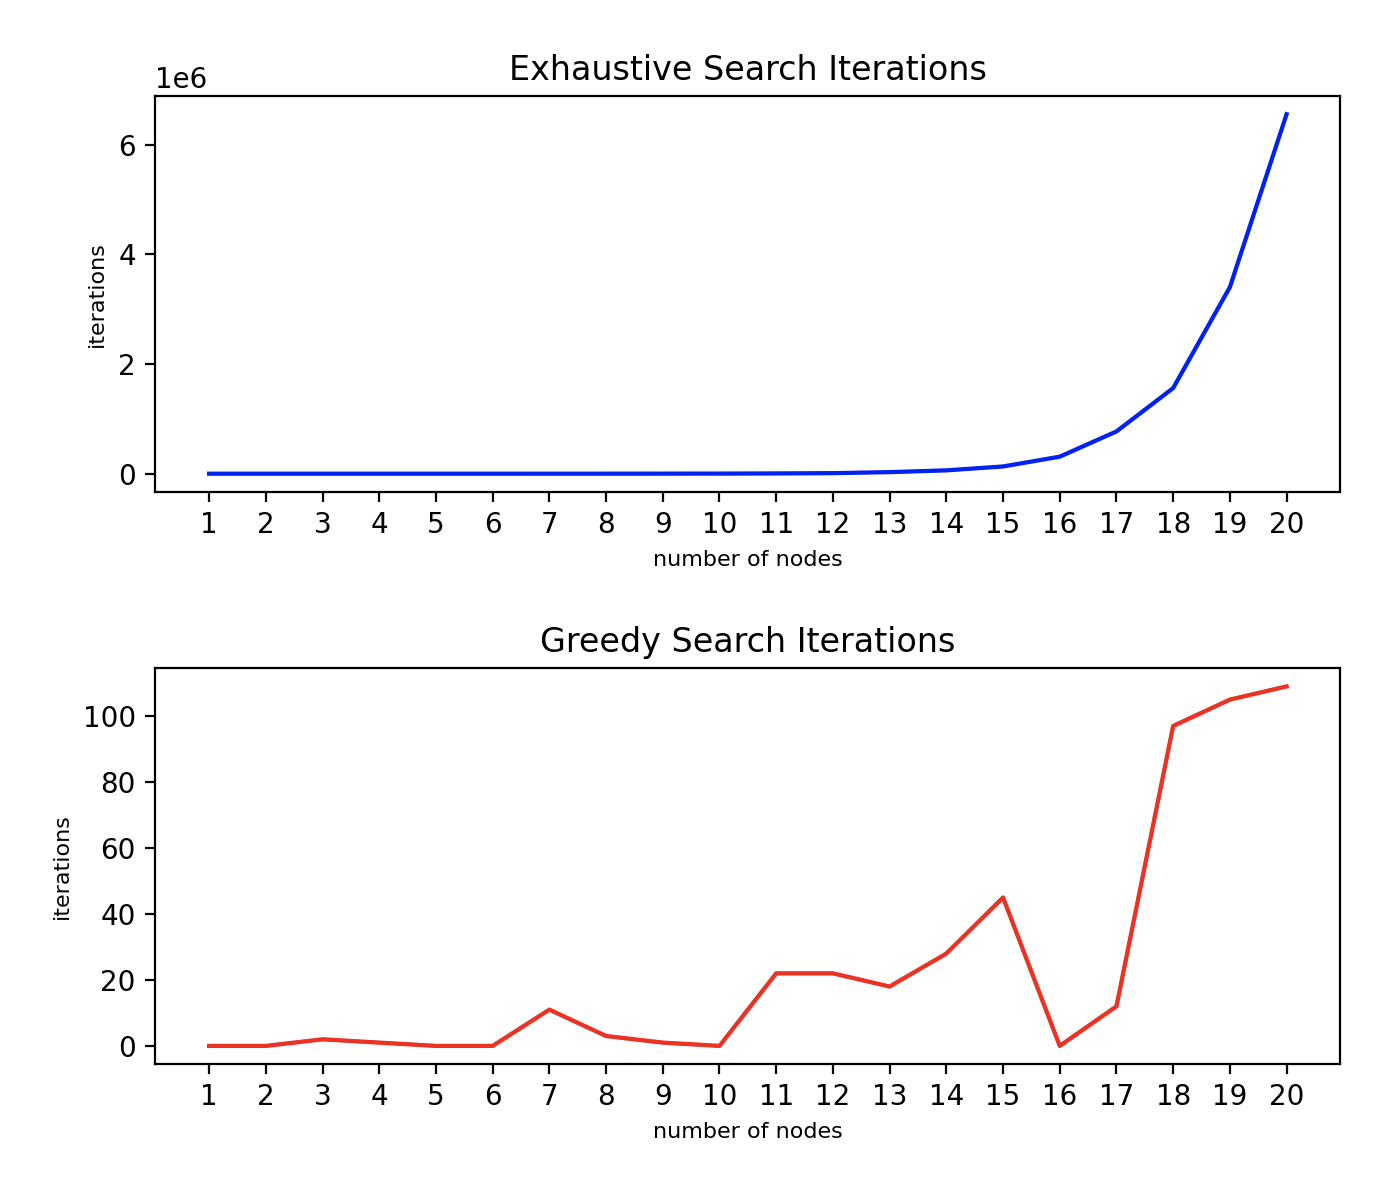
\includegraphics[width=0.9\columnwidth]{./figures/iterations_0.125.png}
    \caption{Iterations on the Exhaustive and Greedy Algorithms}
    \label{fig: Iterations on the Exhaustive and Greedy Algorithm}
\end{figure}

Comparing the two algorithms, as seen in the plot above, the number of iterations/operations increases exponentially using the exhaustive search algorithm, and it is much larger than the same value obtained when using the greedy search. This happens because, as explained in the computational analysis, the exhaustive algorithm performs more operations, mainly when computing the power set of the nodes' set. Also, the greedy approach returns the first solution found, it may not be the optimal one, but this translates into much fewer calculations in comparison to the exhaustive approach. Another thing to notice is that, as these graphs were randomly generated, in most of the cases, it will be impossible to have a solution starting on the node with the lowest weight, other than the set with all nodes. 

\begin{figure}[H]
    \centering
    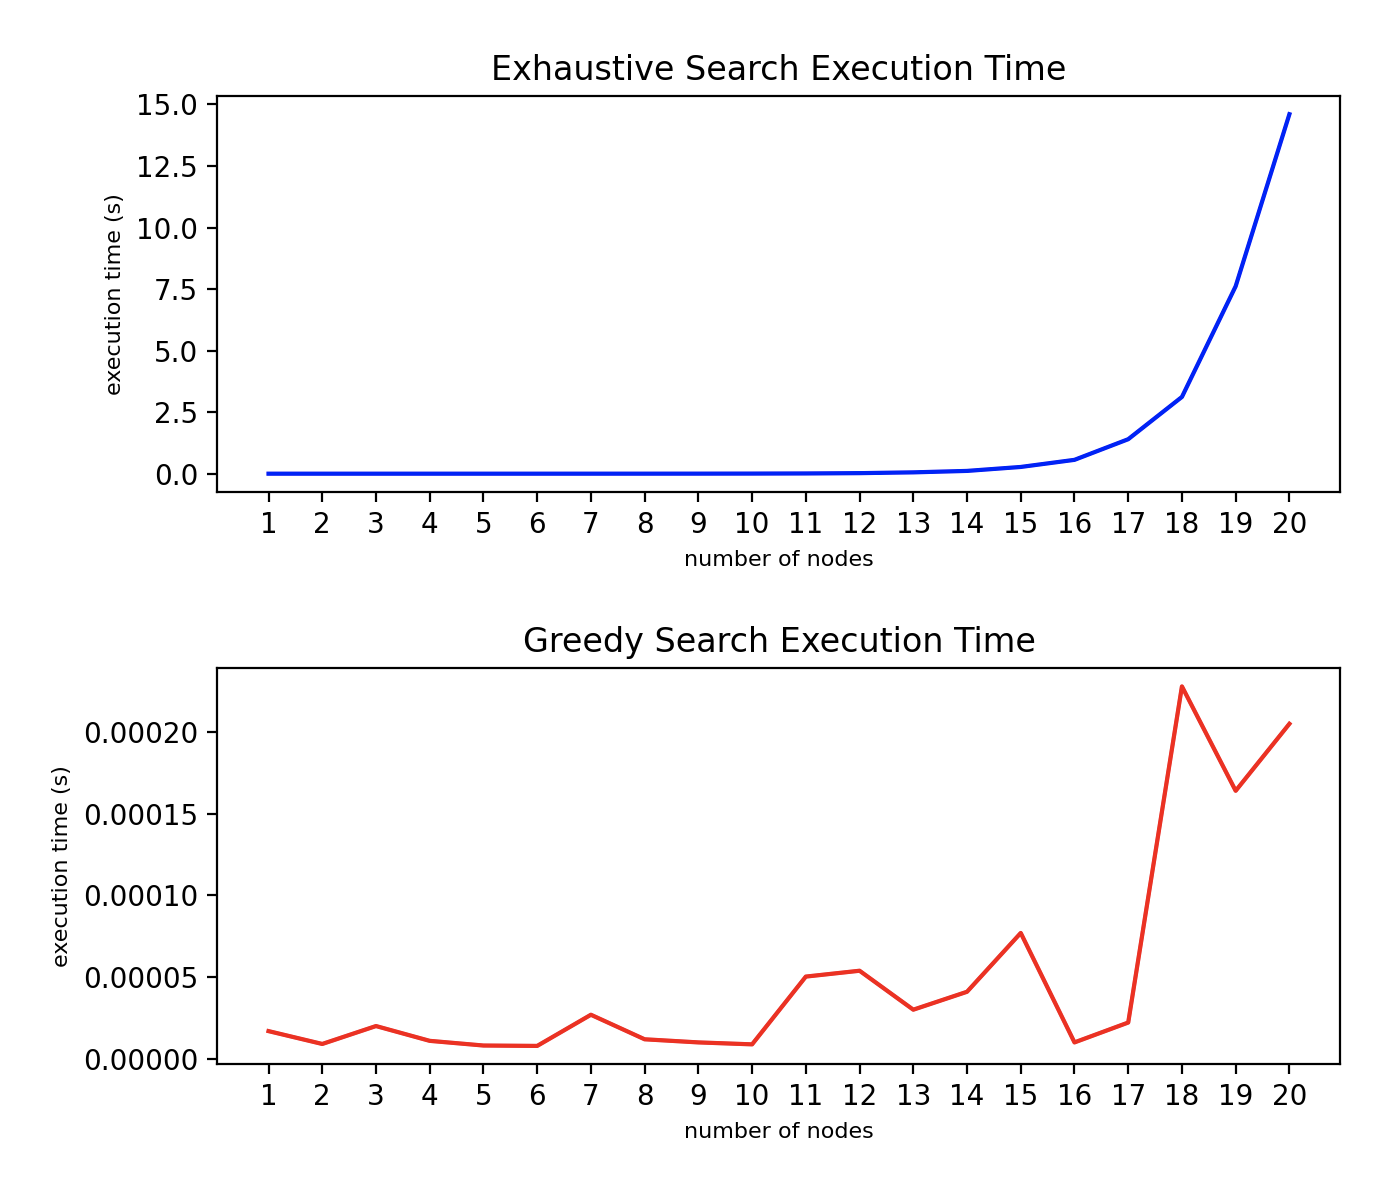
\includegraphics[width=0.9\columnwidth]{./figures/execution_time_number_0.125.png}
    \caption{Execution Time of the Exhaustive and Greedy Algorithms}
    \label{fig: Execution Time of the Exhaustive and Greedy Algorithms}
\end{figure}

As well as the number of iterations, the execution time also increases exponentially when using the exhaustive search, and it is also much larger than the time taken by the greedy search. The explanation is the same that in the previous case. 

\begin{figure}[H]
    \centering
    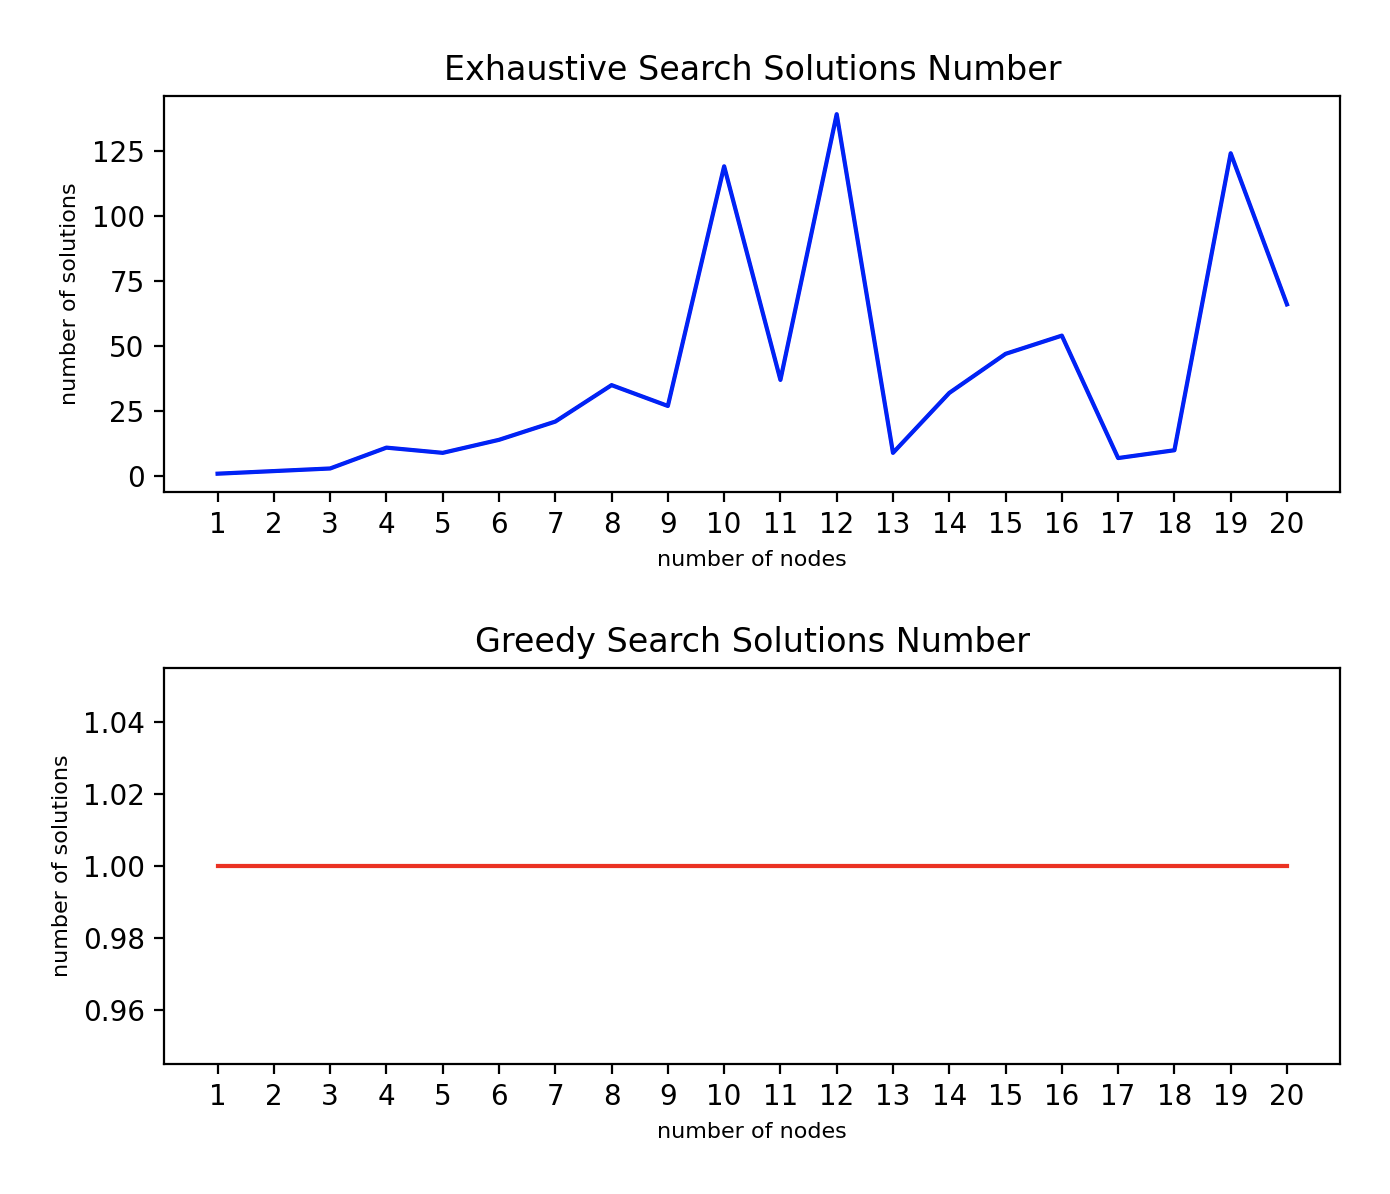
\includegraphics[width=0.9\columnwidth]{./figures/solutions_number_0.125.png}
    \caption{Number of Solutions for the Exhaustive and Greedy Algorithms}
    \label{fig: Number of Solutions for the Exhaustive and Greedy Algorithms}
\end{figure}

Finally, comparing both algorithms regarding the number of solutions found, and as mentioned above, the greedy approach returns the first solution found, therefore, the number of solutions for this algorithm is always 1.

\section{Conclusion}

This assignment allowed a better understanding of the difference between both exhaustive and greedy algorithms. With it can be concluded that, although the exhaustive algorithm always computes the best solution to the minimum weighted closure problem, the computational effort required by this approach is much more compared with the greedy algorithm, with a much larger order, as well as a much larger number of computations, and, finally, a greater complexity. On the contrary, the greedy algorithm computes a solution taking much less time, and iterating also fewer times, but the solution may not be the best one.

\begin{thebibliography}{9}

\bibitem{networkx}
NetworkX developers. (2014-2022). NetworkX. 
\url{https://networkx.org/}

\bibitem{matplotib}
The Matplotlib development team. (2012-2022). Matplotlib. \url{https://matplotlib.org/}

\bibitem{closure_problem}
Wikipedia contributors. (2020, November 25). Closure problem. Wikipedia. \url{https://en.wikipedia.org/wiki/Closure_problem}

\end{thebibliography}




% use a field named url or \url{} for URLs
% Note: the \bibliographystyle is set automatically

\end{document}
